\section{System definition}\label{ch:system-definition}
Let us define the following continuous nonlinear time invariant multiple-input multiple-output system:
\begin{equation}\label{eqn:standard-system}
    \begin{split}
        \dot{x}(t) &= Ax(t) + Bu(t) + E\phi(x) \\
        y_i(t) &= C_ix(t) + Du(t) + v_i(t) + \tau_i(t) \quad i \in \mathcal{N} = \{1,2,\dots,N\}.
    \end{split}
\end{equation}
Where $x \in \mathbb{R}^{n_x}$, $y \in \mathbb{R}^{n_y}$, $u \in \mathbb{R}^{n_u}$ and the nonlinearity $\phi(x) \in \mathbb{R}^{n_{\phi}}$. The $(t)$ indicating time dependency will be omitted from now on. Each $i$ indicates a single output, so each $y_i$ corresponds to a $C_i \in \mathbb{R}^{1 \times n_x}$. The variables without subscript $y$ and $C$, denote all $y_i$ and $C_i$ stacked on top of each other 
$y = 
\begin{bmatrix}
    y_1 & y_2 & \cdots & y_{i} \\
\end{bmatrix}^{T}$ and
$C =
\begin{bmatrix}
    C_1^T & C_2^T & \cdots & C_i^T \\
\end{bmatrix}^{T}$
Let us consider the scenario where an attacker attacks a number of outputs $y_i$, gaining full control the attack signal $\tau_i$. No assumptions are made about $\tau_i$, it can be any unbounded signal. Let us denote the set of attacked outputs as $\mathcal{M} \subset \mathcal{N}$. \\

\subsection{Case study: multi-mass-spring-damper system}
Let us now introduce the system that will be used as a case study: a mass-spring-damper system. This system consists of $b$ mass-spring-dampers in series. Where $x_a,a=1,2,\dots,b$ denotes the position with respect to the previous mass. So the position of a block with respect to the fixed-world is
\begin{equation}\label{eqn:mass-position-wrt-fixed-world}
    \sum^{a}_{j=1}x_j.
\end{equation}
The other variables denote the following: $k_a$ is the spring constant, $c_a$ is the damping constant and $F_a$ is a force acting on the mass.
\begin{figure}[h]
    \centering
    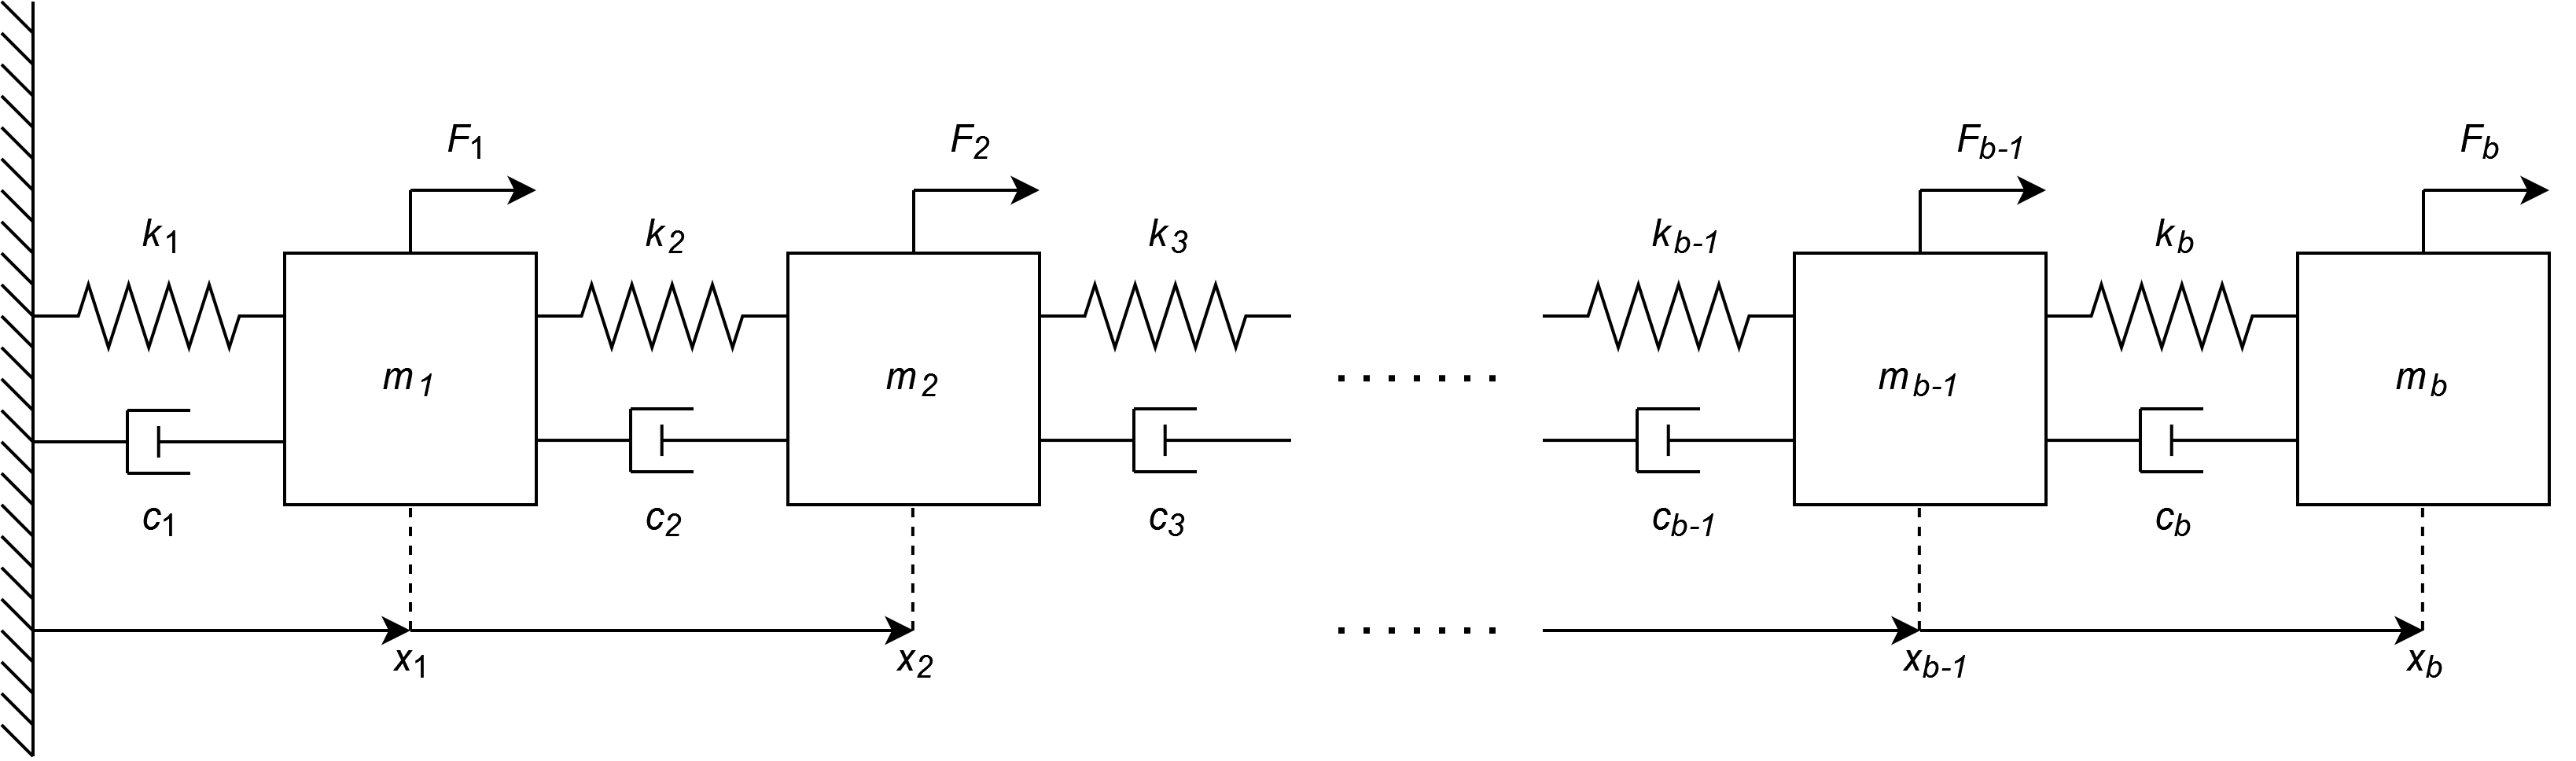
\includegraphics[width=0.9\linewidth]{report/Figures/Mass-spring-damper system.png}
    \caption{Multi-mass-spring-damper system for $b$ mass-spring-dampers in series.}
    \label{fig:mass-spring-damper-system-series}
\end{figure}

We will now derive the state-space form of the system as drawn in \autoref{fig:mass-spring-damper-system-series}. We will start by deriving the equation of motion for the first $b-1$ masses. The sum of forces on a single mass is
\begin{equation}\label{eqn:free-body-equation}
    m_a\ddot{x}_a = F_a - F_s(x_a,k_a,\eta_a) - F_d(\dot{x}_a,c_a) + F_s(x_{a+1},k_{a+1},\eta_{a+1}) + F_d(\dot{x}_{a+1},c_{a+1}).
\end{equation}
Let us now define the spring and damping forces $F_s(x_a)$ and $F_d(\dot{x}_a)$ respectively
\begin{equation*}
    F_s(x_a,k_a,\eta_a) = k_ax_a + k_a \eta_a^2 x_a^3, \quad F_d(\dot{x}_a,c_a) = c_a\dot{x}_a.
\end{equation*}
The formula for the nonlinear spring force is taken from the hardening spring example in \cite[Section 1.2.3]{Khalil2002NonlinearSystems}, the damping force is linear. The expressions for the spring force and damping force will be written as $F_s(x_a)$ and $F_d(\dot{x}_a)$ respectively, where the constants $k_a$, $\eta_a$ and $c_a$ are implicitly passed to the function. $F_s$ will be separated into a linear and nonlinear part as
\begin{equation}\label{eqn:nonlinear-spring}
    \begin{split}
        F_s(x_a) &= F_s^L(x_a) + F_s^{NL}(x_a) \\
        F_s^L(x_a) &= k_ax_a \quad , F_s^{NL}(x_a) = k_a\eta_a^2x^3_a
    \end{split}    
\end{equation}

We will now further simplify equation \eqref{eqn:free-body-equation}, with the split up $F_s$ as in equation \eqref{eqn:nonlinear-spring}

\begin{equation*}
    m_1\Ddot{x}_1 = u_1 - k_1x_1 - c_1\dot{x}_1 + k_2x_2 + c_2\dot{x}_2 - F_s^{NL}(x_1) + F_s^{NL}(x_2), \quad u_1 = F_1,
\end{equation*}
which can be rewritten into
\begin{equation}\label{eqn:mass-spring-damper-first-mass-eom}
    \Ddot{x}_1 = -\frac{k_1}{m_1}x_1 -\frac{c_1}{m_1}\dot{x}_1 + \frac{k_2}{m_1}x_2 + \frac{c_2}{m_1}\dot{x}_2 + \frac{u_1}{m_1} - \frac{F_s^{NL}(x_1)}{m_1} + \frac{F_s^{NL}(x_2)}{m_1}.
\end{equation}
Doing this for the second mass gives the following result:
\begin{equation*}
    \Ddot{x}_2 = -\frac{k_2}{m_2}x_2 - \frac{c_2}{m_2}\dot{x}_2 + \frac{k_3}{m_2}x_3 + \frac{c_3}{m_2}\dot{x}_3 + \frac{u_2}{m_2} - \frac{F_s^{NL}(x_2)}{m_1} + \frac{F_s^{NL}(x_3)}{m_1}.
\end{equation*}
which can be generalised into
\begin{equation}\label{eqn:mass-spring-damper-centre-mass-eom}
    \Ddot{x}_a =  -\frac{k_a}{m_a}x_a - \frac{c_a}{m_a}\dot{x}_a + \frac{k_{a+1}}{m_a}x_{a+1} + \frac{c_{a+1}}{m_a}\dot{x}_{a+1} + \frac{u_a}{m_a} - \frac{F_s^{NL}(x_a)}{m_a} + \frac{F_s^{NL}(x_{a+1})}{m_a}.
\end{equation}
which holds for $a \in \{2,3,\dots,b-2,b-1\}$. Now only the last mass remains
\begin{equation}\label{eqn:mass-spring-damper-last-mass-eom}
    \Ddot{x}_b = -\frac{k_b}{m_b}x_b - \frac{c_b}{m_b}\dot{x}_b + \frac{u_b}{m_b} - \frac{F_s^{NL}(x_b)}{m_b}
\end{equation}

Let us now define the state vector $x$ from equation \eqref{eqn:standard-system} as
\begin{equation}\label{eqn:msd-x}
    x =
    \begin{bmatrix}
        x_1 & \dot{x}_1 & x_2 & \dot{x}_2 & \cdots & x_b & \dot{x}_{b}
    \end{bmatrix}^T
\end{equation}
Using equations \eqref{eqn:mass-spring-damper-first-mass-eom}\eqref{eqn:mass-spring-damper-centre-mass-eom}\eqref{eqn:mass-spring-damper-last-mass-eom} can now be used to construct the $A$ and $B$ matrices in equation \eqref{eqn:standard-system}
\begin{equation}\label{eqn:msd-A}
    A =
    \begin{bmatrix}
        0 & 1 & 0 & 0 & 0 & 0 & \cdots & 0 & 0 & 0 & 0 \\
        -\frac{k_1}{m_1} & -\frac{c_1}{m_1} & \frac{k_2}{m_1} & \frac{c_2}{m_1} & 0 & 0 & \cdots & 0 & 0 & 0 & 0 \\
        0 & 0 & 0 & 1 & 0 & 0 & \cdots & 0 & 0 & 0 & 0 \\
       0 & 0 & -\frac{k_2}{m_2} & -\frac{c_2}{m_2} & \frac{k_3}{m_2} & \frac{c_3}{m_2} & \cdots & 0 & 0 & 0 & 0 \\
        \vdots & \vdots & \vdots & \vdots & \vdots & \vdots & \ddots & \vdots & \vdots & \vdots & \vdots \\
        0 & 0 & 0 & 0 & 0 & 0 & \cdots & 0 & 0 & 0 & 1 \\
        0 & 0 & 0 & 0 & 0 & 0 & \cdots & 0 & 0 & -\frac{k_b}{m_b} & -\frac{c_b}{m_b} \\
    \end{bmatrix}
\end{equation}
and
\begin{equation}\label{eqn:msd-B}
    B = 
    \begin{bmatrix}
        0 & 0 & \cdots & 0 \\
        \frac{1}{m_1} & 0 & \cdots & 0 \\
        0 & 0 & \cdots & 0 \\
        0 & \frac{1}{m_2} & \cdots & 0 \\
        \vdots & \vdots & \ddots & \vdots \\
        0 & 0 & \cdots & 0 \\
        0 & 0 & \cdots & \frac{1}{m_b} \\
    \end{bmatrix}.
\end{equation}
Let us now derive the nonlinear contributions $\phi$ and $E$ from equation \eqref{eqn:standard-system} from equations \eqref{eqn:mass-spring-damper-first-mass-eom}\eqref{eqn:mass-spring-damper-centre-mass-eom}\eqref{eqn:mass-spring-damper-last-mass-eom}.
\begin{equation}
    \phi(x) =
    \begin{bmatrix}
        F_s^{NL}(x_1) & F_s^{NL}(x_2) & \cdots & F_s^{NL}(x_b)
    \end{bmatrix}
\end{equation}
and
\begin{equation}
    E =
    \begin{bmatrix}
        0 & 0 & 0 & \cdots & 0 \\
        -\frac{1}{m_1} & \frac{1}{m_1} & 0 & \cdots & 0 \\
        0 & 0 & 0 & \cdots & 0 \\
        0 & -\frac{1}{m_2} & \frac{1}{m_2} & \cdots & 0 \\
        \vdots & \vdots & \vdots & \ddots & \vdots \\
        0 & 0 & 0 & \cdots & 0 \\
        0 & 0 & 0 & \cdots & -\frac{1}{m_b} \\
    \end{bmatrix}.
\end{equation}

We will now construct the $C$ matrix, in order to do so let us note that only the absolute positions \eqref{eqn:mass-position-wrt-fixed-world} of each mass are measured. This leads to
\begin{equation}\label{eqn:msd-C}
    C = 
    \begin{bmatrix}
        1 & 0 & 0 & 0 & \cdots & 0 & 0 & 0 & 0 \\
        1 & 0 & 1 & 0 & \cdots & 0 & 0 & 0 & 0 \\
        \vdots & \vdots & \vdots & \vdots & \ddots & \vdots & \vdots & \vdots & \vdots \\
        1 & 0 & 1 & 0 & \cdots & 1 & 0 & 0 & 0 \\
        1 & 0 & 1 & 0 & \cdots & 1 & 0 & 1 & 0 \\
    \end{bmatrix}
\end{equation}
where each row is a single output. In this system the $D$ matrix is equal to $0$.\\ 
\textcolor{red}{note on observability?}